\documentclass[../main.tex]{subfiles}
\begin{document}
\chapter{AFM - SNOM}
Le immagini prese in esame in questa tesi sono state prodotte con un microscopio NeaSNOM. In questo capitolo viene descritta la sua struttura e le sue modalità di funzionamento...
\change{Imposta una introduzione quando finisci il capitolo}
\section{Storia della Microscopia}

I primi microscopi composti costruiti risalgono al 17\textdegree\ secolo, oltre 400 anni fa. È in quest'epoca che si riuscì a vedere per la prima volta i microrganismi che abitano la Terra ed ebbe inizio lo studio della Microbiologia. \textit{Robert Hooke} osservò le pareti cellulari e usò per la prima volta il termine ``cellula" \cite{fara_2009, micrographia}, mentre \textit{Antoine van Leeuwenhoek} sviluppò dei microscopi semplici (a singola lente) con ingrandimenti molto superiori a quelli degli strumenti contemporanei e fu il primo ad osservare microrganismi, come batteri e globuli rossi.\cite{lane_2015, dobell_1923, corliss_1975, jessup_2024}

\subsection{Microscopio ottico composto}

Il microscopio ottico composto ingrandisce l'immagine del campione usando delle lenti. il campione può essere illuminato facendolo attraversare dalla luce sul lato opposto all'obiettivo (microscopia a luce trasmessa) oppure riflettendocela sopra (microscopia a luce riflessa).

Il sistema più semplice è composto da due lenti, una lente obiettivo vicina al campione da esaminare, e una lente oculare vicina all'osservatore. Il campione è prima messo a fuoco dalla lente obiettivo dentro al microscopio in una immagine reale, poiché è creata dalla convergenza dei raggi di luce, poi questa immagine viene nuovamente ingrandita dalla lente oculare che crea una nuova immagine, stavolta virtuale visto che è creata da proiezioni di raggi divergenti. L'osservatore quindi vedrà un'immagine ingrandita, invertita e virtuale del campione esaminato.

\begin{figure}[h]
\centering
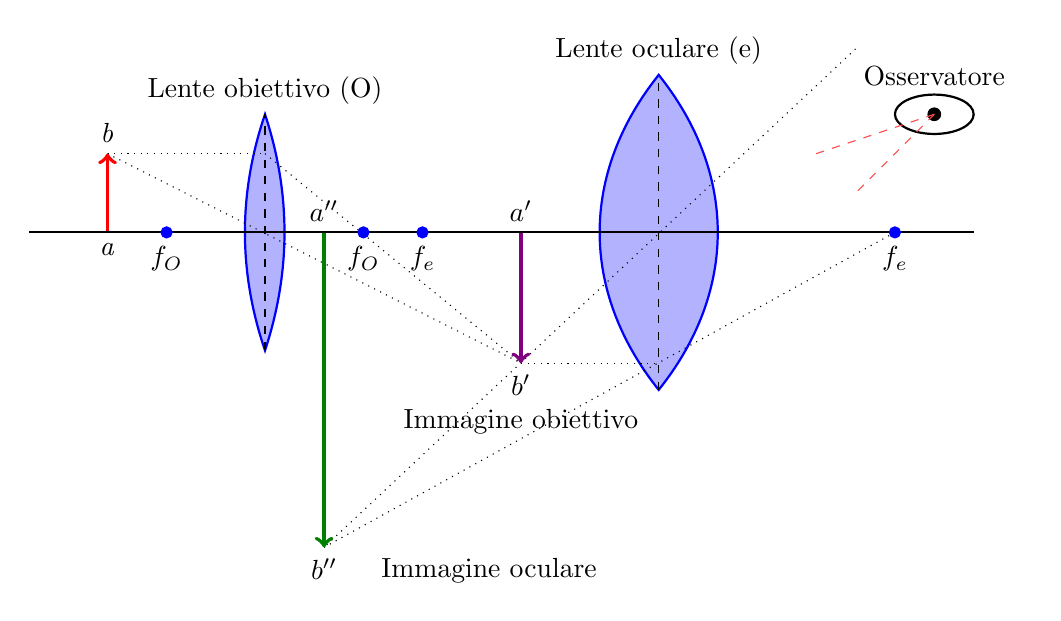
\begin{tikzpicture}
	% lente obiettivo
	\filldraw[thick,blue!30, draw=blue] (3,1.5) 
		.. controls (2.66,0.5) and (2.66,-0.5) .. (3,-1.5)
		.. controls (3.33,-0.5) and (3.33,0.5) .. cycle
		node[black,above] {Lente obiettivo (O)};
	\draw[dashed] (3,-1.5) -- (3,1.5);
	
	% lente oculare
	\filldraw[thick,blue!30, draw=blue] (8,2) 
	.. controls (9,0.75) and (9,-0.75) .. (8,-2)
	.. controls (7,-0.75) and (7,0.75) .. cycle
	node[black,above] {Lente oculare (e)};
	\draw[dashed] (8,-2) -- (8,2);
			
	\draw[dotted] (1,1) -- (3,1);
	\draw[dotted] (3,1) -- (6.25,-1.66);
	\draw[dotted] (1,1) -- (6.25,-1.66);
	
	\draw[dotted] (6.25,-1.66) -- (8,-1.66);
	\draw[dotted] (11,0) -- (3.75,-4);
	\draw[dotted] (10.5,2.33) -- (3.75,-4);
	
	% ogetto
	\draw[line width=0.5mm,Red,->] (1,0) node[below, black] {\textit{a}}
		-- (1,1) node[above, black] {\textit{b}};
	
	% immagine reale
	\draw[line width=0.5mm,Purple,->] (6.25,0) node[above, black] {$a'$}
		-- (6.25,-1.66) node[below, black, align=center] {$b'$ \\ \text{Immagine obiettivo}};

	% immagine virtuale
	\draw[line width=0.5mm,Green,->] (3.75,0) node[above, black] {$a''$}
		-- (3.75,-4) node[below, black] {$b''$} node[below right, black] {\ \ \quad Immagine oculare};

	% linea principale
	\draw[thick] (0,0) -- (12,0);
	
	% lungheazza focale lente oculare
	\filldraw[blue] (5,0) circle (2pt) node[below,black,inner sep=5pt]{$f_e$};
	\filldraw[blue] (11,0) circle (2pt) node[below,black,inner sep=5pt]{$f_e$};
	
	% lungheazza focale lente obiettivo
	\filldraw[blue] (1.75,0) circle (2pt) node[below,black,inner sep=5pt]{$f_O$};
	\filldraw[blue] (4.25,0) circle (2pt) node[below,black,inner sep=5pt]{$f_O$};
	
	% occhio
	\draw[thick] (11.5,1.5) ellipse (0.5 and 0.25)
		node[above, inner sep=10pt] {Osservatore};
	
	% pupilla
	\filldraw[black] (11.5,1.5) circle (0.08);
	
	% raggi visivi
	\draw[red!70, dashed] (11.5,1.5) -- (10,1);
	\draw[red!70, dashed] (11.5,1.5) -- (10.5,0.5);
\end{tikzpicture}
\caption{Principio di funzionamento di un microscopio ottico composto}
\label{fig:com_diag}
\end{figure}

Il microscopio ottico composto ha continuato ad essere sviluppato fino ad oggi e ne sono state create molte varianti per scopi più specializzati, come il microscopio a contrasto di fase (\acrshort{pcm})\cite{zernike_1955} o il microscopio confocale (\acrshort{clsm})\cite{pawley_2006}. In generale, oggi la microscopia ottica ha raggiunto altissimi livelli di prestazioni, sia ottiche che meccaniche, ma la cui risoluzione spaziale è rimasta bloccata dal limite di diffrazione della luce.

\subsection{Apertura numerica}

Il primo a definire questo limite fu \textit{Ernst Abbe} nel 1881, anno in cui pubblicò il suo lavoro sulla misura dell'apertura dei microscopi.\cite{abbe_1881} Questo limite, chiamato apertura numerica (\acrshort{na}), si basa sull'intervallo degli angoli con cui la luce può entrare o uscire dal microscopio  ed è comunemente usato in microscopia come parametro delle ottiche per valutarne la risoluzione. Questo numero è definito come il prodotto tra l'indice di rifrazione \textit{n} e il seno dell'apertura angolare della lente.

\begin{equation}
	\mathit{NA}=n\sin\theta
\end{equation}

Da questa formula, Abbe continuò il suo lavoro arrivando a definire anche la distanza minima tra due elementi diversi affinchè si possano apprezzare attraverso un microscopio.\cite{abbe_1882}

\begin{equation}
d=\frac{\lambda}{2\mathit{NA}}=\frac{\lambda}{2n\sin\theta}
\end{equation}

Usando l'aria come mezzo di trasmissione si ha un indice di rifrazione di 1, mentre si può arrivare fino a circa 1.5 immergendo il campione e l'obiettivo in olio. Per quanto riguarda l'apertura angolare massima,  teoricamente può arrivare fino a 180\degree, il che si traduce in un valore di $\theta=90$\degree, ma ad ora le lenti con la più alta apertura angolare mai realizzate si fermano approssimativamente a 144\degree, che corrisponde a un valore di $\sin\left(\theta=72\degree\right) \approx 0.95$.\cite{leica_aperture}\\

\begin{figure}[h]
\centering
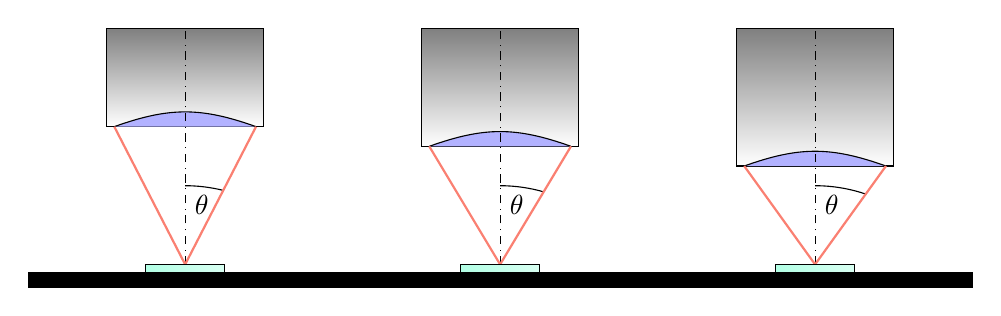
\begin{tikzpicture}
	%primo obiettivo
	\shadedraw (1,1.75) -- (1,3) -- (3,3) --(3,1.75) -- cycle;
	\filldraw[blue!30, draw=black] (1.1,1.75) 
		.. controls (1.8,2) and (2.2,2) 
		.. (2.9,1.75);
	\draw[dash dot] (2,0) -- (2,3);
	\draw (2,1) node[below right]{$\theta$} arc (90:76:2);
	\draw[Salmon, thick] (1.1,1.75) -- (2,0) -- (2.9,1.75);
	\shadedraw[left color=Aquamarine!60, right color=Aquamarine!30] (1.5,0) rectangle (2.5,-0.1);
	
	%secondo obiettivo
	\shadedraw (5,1.5) -- (5,3) -- (7,3) --(7,1.5) -- cycle;
	\filldraw[blue!30, draw=black] (5.1,1.5) 
	.. controls (5.8,1.75) and (6.2,1.75) 
	.. (6.9,1.5);
	\draw[dash dot] (6,0) -- (6,3);
	\draw (6,1) node[below right]{$\theta$} arc (90:74:2);
	\draw[Salmon, thick] (5.1,1.5) -- (6,0) -- (6.9,1.5);
	\shadedraw[left color=Aquamarine!60, right color=Aquamarine!30] (5.5,0) rectangle (6.5,-0.1);
	
	%terzo obiettivo
	\shadedraw (9,1.25) -- (9,3) -- (11,3) --(11,1.25) -- cycle;
	\filldraw[blue!30, draw=black] (9.1,1.25) 
	.. controls (9.8,1.5) and (10.2,1.5) 
	.. (10.9,1.25);
	\draw[dash dot] (10,0) -- (10,3);
	\draw (10,1) node[below right]{$\theta$} arc (90:71:2);
	\draw[Salmon, thick] (9.1,1.25) -- (10,0) -- (10.9,1.25);
	\shadedraw[left color=Aquamarine!60, right color=Aquamarine!30] (9.5,0) rectangle (10.5,-0.1);
	
	%base
	\fill[black] (0,-0.1) rectangle (12,-0.3);
\end{tikzpicture}
\caption{Obiettivi con diverse aperture}
\label{fig:na_diag}
\end{figure}

Per migliorare la risoluzione oltre il limite dei 250nm, ottenibili usando lunghezze d'onda dello spettro visibile, si possono scegliere onde eletttromagnetiche a lunghezza minore, come i raggi X o UV, oppure raggi di altra natura, come i fasci di elettroni. Queste tecniche portano una risoluzione maggiore ma anche delle controindicazioni, come una scarsa risposta da parte del campione oppure tossicità.\cite{hell_2007}

\subsection{Microscopio elettronico}

La scoperta che i raggi di elettroni si comportano come onde con lunghezze d'onda più corte della luce visibile aprì nuove opportunità. I primi esemplari furono sviluppati nel 1931 da \textit{Max Knoll} e \textit{Ernst Ruska}\cite{oatley1982early} e già due anni dopo furono in grado di apprezzare dettagli oltre il limite dei microscopi ottici tradizionali.\cite{physics_nobel} 

I microscopi elettronici utilizzano un fascio di elettroni al posto della luce e delle lenti magnetiche invece che ottiche. Usando raggi di elettroni invece che di luce, questi microscopi non misurano l'interazione tra materia e luce ma tra materia ed elettroni, aprendo le porte a nuovi campi di studio. 

Nei primi microscopi elettronici, il campione da esaminare è posto tra il cannone elettronico e il rilevatore e l'immagine si forma in base a come gli elettroni vengono trasmessi attraverso il campione, che deve essere molto sottile (meno di 100nm). Questo tipo di microscopi si chiama microscoio elettronico \textit{a trasmissione} (\acrshort{tem}) e i modelli più recenti possono arrivare a risoluzioni spaziali fino a 0.5\AA\ (50pm).\cite{rolf_2009}

Un altro tipo molto usato di microscopi elettronici è quello \textit{a scansione} (\acrshort{sem}), in cui non si rileva il fascio trasmesso attraverso il campione bensì i raggi secondari che sono generati dalla loro interazione (come elettroni secondari o raggi X). Questa tecnica può ottenere immagini tridimenzionali e non richiede un campione sottile quanto la \acrshort{tem} ma deve essere conduttivo e messo a terra, o comunque ricoperto da un film metallico. Modelli recenti di \acrshort{sem} possono arrivare a risoluzioni spaziali fino a 0.4nm.\cite{hitachi_sem}

\begin{figure}[htbp]
\centering
\begin{subfigure}[t]{4.5cm}
	\centering
	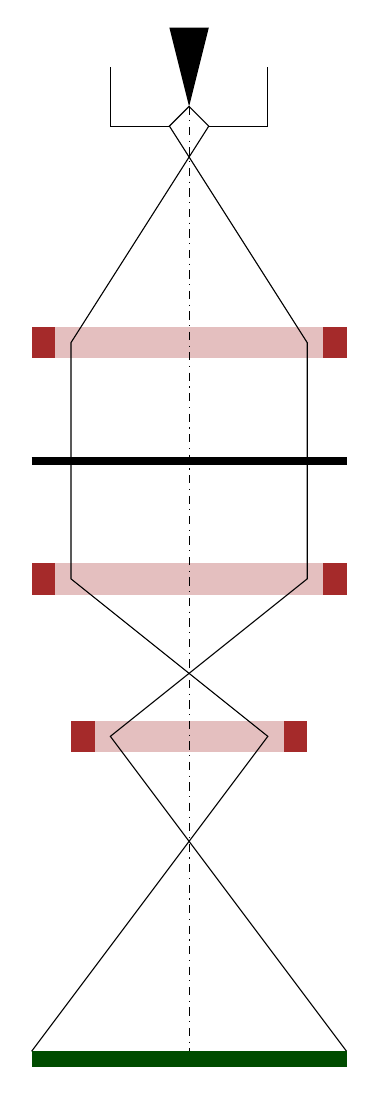
\begin{tikzpicture}
		%cannone
		\fill (1.75,1) -- (2,0) -- (2.25,1) -- cycle;
		\draw (1,0.5) -- (1,-0.25) -- (1.75,-0.25);
		\draw (3,0.5) -- (3,-0.25) -- (2.25,-0.25);
		
		% condensatore
		\fill[Brown] (0.3,-3.2) rectangle (0,-2.8);
		\fill[Brown] (3.7,-3.2) rectangle (4,-2.8);
		\fill[Brown!30] (0.3,-3.2) rectangle (3.7,-2.8);
		
		%obiettivo
		\fill[Brown] (0.3,-6.2) rectangle (0,-5.8);
		\fill[Brown] (3.7,-6.2) rectangle (4,-5.8);
		\fill[Brown!30] (0.3,-6.2) rectangle (3.7,-5.8);
		
		%proiettore
		\fill[Brown] (0.8,-8.2) rectangle (0.5,-7.8);
		\fill[Brown] (3.2,-8.2) rectangle (3.5,-7.8);
		\fill[Brown!30] (0.8,-8.2) rectangle (3.2,-7.8);
		
		\draw (2,0) -- (1.75,-0.25) -- (3.5,-3) -- (3.5,-6) -- (1,-8) -- (4,-12);
		\draw (2,0) -- (2.25,-0.25) -- (0.5,-3) -- (0.5,-6) -- (3,-8) -- (0,-12);

		\draw[line width=1mm] (0,-4.5) -- (4,-4.5);

		\draw[dash dot] (2,0) -- (2,-12);
		\fill[Green!60!Black] (0,-12) rectangle (4,-12.2);
	\end{tikzpicture}
	\caption{TEM}
\end{subfigure}
\hfill
\begin{minipage}[t]{0.3\textwidth}
	\centering
	\vspace{-12.4cm} Cannone elettronico\\
	\vspace{2.6cm} Lente condensatore\\
	\vspace{1.05cm} Campione\\
	\vspace{1.05cm} Lente obiettivo\\
	\vspace{0.525cm} Bobina di scansione\\
	\vspace{0.525cm} Lente proiettore\\
	\vspace{2cm} Campione\\
	\vspace{1.05cm} Camera CCD\\
\end{minipage}%
\begin{subfigure}[t]{5cm}
	\centering
	\begin{tikzpicture}
		%cannone
		\fill (1.75,1) -- (2,0) -- (2.25,1) -- cycle;
		\draw (1,0.5) -- (1,-0.25) -- (1.75,-0.25);
		\draw (3,0.5) -- (3,-0.25) -- (2.25,-0.25);
		
		% condensatore
		\fill[Brown] (0.3,-3.2) rectangle (0,-2.8);
		\fill[Brown] (3.7,-3.2) rectangle (4,-2.8);
		\fill[Brown!30] (0.3,-3.2) rectangle (3.7,-2.8);
		
		% deflettore
		\fill[Blue] (1.7,-6.2) rectangle (1.4,-5.8);
		\fill[Blue] (2.3,-6.2) rectangle (2.6,-5.8);
		\fill[Blue!30] (1.7,-6.2) rectangle (2.3,-5.8);
		
		%proiettore
		\fill[Brown] (0.8,-8.2) rectangle (0.5,-7.8);
		\fill[Brown] (3.2,-8.2) rectangle (3.5,-7.8);
		\fill[Brown!30] (0.8,-8.2) rectangle (3.2,-7.8);
		
		%campione
		\draw (2.5,-9.6) -- (1.2,-10) -- (2,-11.2) -- (3.3,-10.8) -- cycle;
		\coordinate (A) at (2.5,-9.6);
		\coordinate (B) at (1.2,-10);
		\coordinate (C) at (2,-11.2);
		\coordinate (D) at (3.3,-10.8);
		\foreach \t in {0.125,0.25,...,0.875} {
			\path 
        		coordinate (L) at ($(B)!\t!(A)$)
				coordinate (R) at ($(C)!\t!(D)$);
			\draw[red, dashed, ->] (L) -- (R);
		};
		
		\draw (2,0) -- (1.75,-0.25) -- (3.5,-3) -- (1,-8) -- (2,-10);
		\draw (2,0) -- (2.25,-0.25) -- (0.5,-3) -- (3,-8) -- (2,-10);
				
		%indicazioni
		\draw (1.5,-6) -- (-0.5,-7.1);
				
		\draw[dash dot] (2,0) -- (2,-10);
		\fill[transparent] (0,-12.2){};
	\end{tikzpicture}
	\caption{SEM}
\end{subfigure}%
\caption{Principio di funzionalento dei microscopi TEM e SEM}
\label{fig:em_diag}
\end{figure}

\subsection{Microscopio a effetto tunnel}

La branca di microscopia di cui fa parte quello di interesse in questa tesi è lam microscopia a scansione di sonda (\acrshort{spm}) e fu fondata nel 1981 con l'invenzione del microscopio a effetto tunnel (\acrshort{stm}).\cite{ieee_spm} 
Questi microscopi rilevano la superficie del campione usando una punta minuscola su cui è imposta una differenza di potenziale con il piano di osservazione. Mantenendo l'altezza della punta costante, si può misurare direttamente la variazione di corrente attraverso il campione in movimento, mentre per misurarne l'altezza si può matenere costante la corrente e applicareun feedback al motore piezoelettrico che regola l'altezza della punta. Avendo una risoluzione di 0.1nm, questa tecnica permette di osservare singoli atomi, ma può essere usata solo se il campione è conduttivo.\cite{bai_2000}

\begin{figure}[h]
\centering
\begin{tikzpicture}
	% punta
	\filldraw[fill=gray] (-0.25,0) -- (-0.25,-1.75) -- (0,-2.5) -- (0.25,-1.75) 
		node[right, xshift=3mm] {Punta}
		-- (0.25,0);
	
	% sistema di controllo
	\fill (-2.5,-1.9) rectangle (-2.45,-1.6);
	\fill (-2.4,-2.1) rectangle (-2.35,-1.4);
	\fill (-2.3,-1.9) rectangle (-2.25,-1.6);
	\fill (-2.2,-2.1) rectangle (-2.15,-1.4);
	\fill (-2.1,-1.9) rectangle (-2.05,-1.6);
	\fill (-2.0,-2.1) rectangle (-1.95,-1.4);
	\draw (-1.95,-1.75) node[above right] {\textbf{+}}
		-- (-0.25,-1.75);
	\draw (-2.5,-3.6) -- (-3,-3.6) -- (-3,-1.75) -- (-2.5,-1.75);
	\draw (-3,-2.75) -- (-5,-2.75) -- (-5, 0);
	\filldraw[fill=white] (-3,-2.75) circle (0.33)
		node[below left, xshift=-3mm, yshift=-3mm] {Amperometro};
	\draw[->] (-3.15,-2.9) -- (-2.85,-2.6);
	\draw[->] (-5,0) -- (-1,0);
	\node[draw, fill=white, align=center] at (-5,0) {Elettronica\\di controllo};
	
	% cilindro
	\node[cylinder, minimum height=2.5cm, minimum width=2cm, rotate=90, draw,
		shading=axis, left color=gray!30, right color=gray!60, middle color=gray!10] {};
	\filldraw[fill=white] (0,1.225) ellipse (1cm and 0.12cm)
		node[right, xshift=13mm] {Scanner};
	
	\draw[<->, thick] (1,1.5) -- (-1,1.5) node[midway, above] {X,Y};
	
	\draw (1,0)
		node[right, xshift=3mm] {Motore piezoelettrico}
		.. controls (1,-0.2) and (-1,-0.2) .. (-1,0);
	
	\draw[<->, thick] (0,-0.2) -- (0,-1.1) node[midway, right] {Z};
	
	% campione
	\filldraw[fill=purple] (-2,-3.5) -- (-2,-3.25)
		.. controls (-2,-3) and (-1.33,-3) .. (-1.25,-3.25)
		.. controls (-1,-3.3) and (-0.5, -2.9) .. (0.25,-3.25)
		.. controls (0.75,-3.4) and (1,-3.1) .. (1.7,-3.25)
		.. controls (1.8, -3.2) and (1.9, -3) .. (2,-3)
	 	-- (2,-3.5) node[above right, xshift=3mm] {Campione}
	 	-- cycle;
	 
	 %base
	 \fill (-2.5,-3.5) rectangle (2.5,-3.7);
	 
\end{tikzpicture}
\caption{Principio di funzionamento di un microscopio a effetto tunnel}
\label{fig:stm_di1ag}
\end{figure}

\section{AFM}

\section{SNOM}

\section{Batteri}

\end{document}
